\section{Validación de la Implementación} \label{sec:experimental}

Lo último a realizar fue la validación de las funcionalidades de la aplicación desarrollada. Para ello, se establecieron escenarios de prueba por los cuales se pueda comprobar el funcionamiento de aplicación. Estos, se definieron con el fin de probar la capacidad y la efectividad de los mecanismos implementados de modificar el estado inicial de la aplicación hacia el estado de referencia, al igual que la identificación de algunas de las falencias de esta.

Ahora, se debe resaltar que, las pruebas se realizaron usando un servicio genérico, apodado Mocker, encargado de la generación de datos, especialmente desarrollado para funcionar en condiciones ideales. 

Para cada una de estas pruebas, se definió un estado de referencia, dadas unas condiciones iniciales, y una serie de eventos los cuales modificarán nuevamente el estado de la aplicación, las cuales tendrán que ser nuevamente manejadas.

\subsection{Escenario Experimental A} \label{sec:EscenarioExperimentalA}

El primer escenario, busca el evaluar la capacidad de la implementación realizada de iniciar toda una aplicación desde cero. Partiendo de esto, se definió la aplicación vista en la figura \ref{fig:ExpA}. Esta tiene dos locaciones raíz, con requerimientos de datos iguales en ambas.

\begin{figure}[H]
    \centering
    \caption{\\Diagrama del escenario experimental A}
    \label{fig:ExpA}
    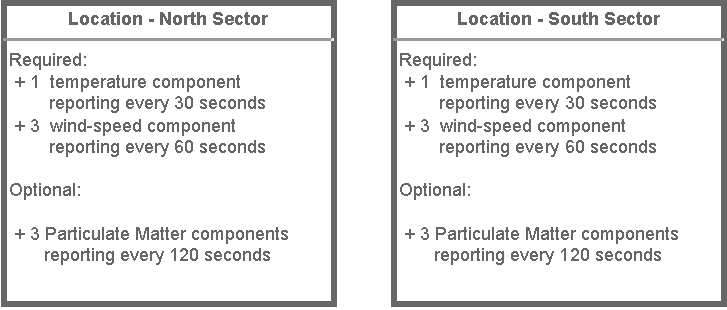
\includegraphics[width=0.8\linewidth]{images/ScenarioA.pdf}
    \vspace{-4mm}
\end{figure}

Inicialmente, no habrán dispositivos presentes en ejecución, por lo que el sistema tendrá que identificar la falla, definir las acciones de adición correspondientes, y ejecutarlas para poder suplir con los requerimientos de datos.

Para ello, tomando como referencia la figura \ref{fig:ExpA}, se realizó la declaración del estado de referencia, presente en el anexo \ref{ape:ExpA}, y, como observa en la figura \ref{fig:ValidA}, se validó usando \textit{Lexical}.

\begin{figure}[H]
    \centering
    \caption{\\Validación de la declaración de referencia realizada para el escenario experimental A}
    \label{fig:ValidA}
    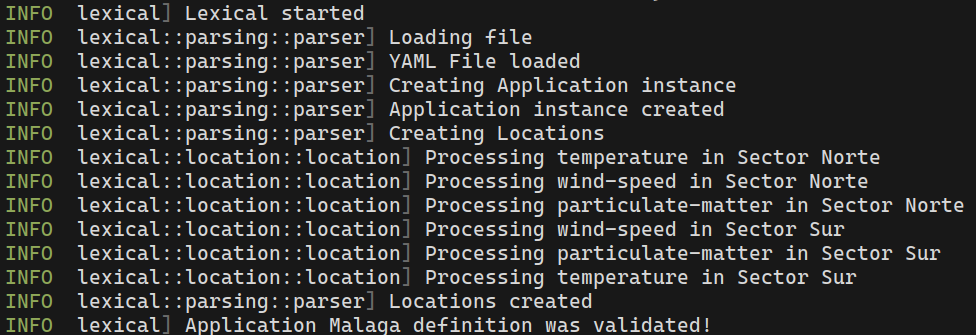
\includegraphics[width=0.7\linewidth]{images/ValidationLexicalA.png}
    \vspace{-4mm}
\end{figure}

Ya con las condiciones iniciales, y el estado de referencia definido, se estructuraron, las directivas, vistas en el anexo \ref{ape:DirectivesA}, que permitirían realizar la adaptación de la arquitectura hacia el estado de objetivo. 

Partiendo de todo lo anterior, se definió la serie de pasos a realizar para este primer escenario experimental:

\begin{enumerate}[itemsep=0mm]
    \item Desplegar los servicios de Smart Campus UIS
    \item Desplegar los servicios \textit{Bran} y \textit{DoThing}.
    \item Usando \textit{Lexical}, establecer el estado de referencia de la aplicación.
    \item Declarar en los endpoints de \textit{Bran}, las directivas definidas.
    \item Desplegar el servicio \textit{Looker} para la aplicación.
    \item A la nivelación del estado de la aplicación.
\end{enumerate}

Al final de la simulación de este escenario, se eliminarán todos los servicios desplegados con el fin de asegurar una ejecución limpia de futuros procesos.


\subsection{Resultados De Escenario Experimental B}

